% file: 3-8-apsp/negative-weight-cycle-k.tex

\documentclass[tikz]{standalone}
\usetikzlibrary{positioning, decorations.pathmorphing}

\begin{document}
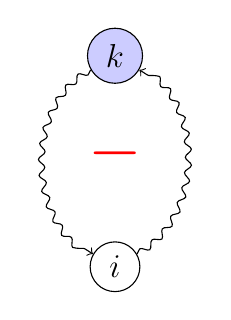
\begin{tikzpicture}[every node/.style = {draw, circle, minimum size = 8pt, font = \large},
    path/.style = {->, decorate, decoration = {snake, amplitude = .4mm, segment length = 2mm, post length = 1mm}}]

  \node (i) {$i$};
  \node (k) [fill = blue!20, above = 2.0cm of i] {$k$};
  \node (nc) [above = 0.5cm of i, draw = none, font = \Huge] {\textcolor{red}{$-$}};

  \draw[path, out = 30, in = -30] (i) to (k);
  \draw[path, out = 210, in = 150] (k) to (i);
\end{tikzpicture}
\end{document}
